\chapter{Schrandere Scholier}

In het vorige hoofdstuk hebben we een leuk spel gemaakt, we kunnen echter ook serieuze applicaties schrijven. Waarschijnlijk vraag je jezelf wel eens af welk cijfer je moet halen voor een toets om een 8 gemiddeld te blijven staan voor een vak. In dit hoofdstuk gaan we hier een hulpmiddel voor ontwikkelen.

We zullen de applicatie stap-voor-stap opbouwen. We maken een begin met de gebruikersinterface in het \menuitem{design} scherm. Daarna zullen we in de \menuitem{Blocks}-editor ervoor zorgen dat de gebruiker cijfers kan invoeren waarmee we vervolgens kunnen gaan rekenen. Tot slot zorgen we ervoor dat de gegevens opgeslagen worden zodat we niet bij elke start opnieuw hoeven te beginnen.

\section{Een nieuw project aanmaken}
We beginnen met het aanmaken van een nieuw project. In hoofdstuk \ref{chap:ontwikkelomgeving} heb je een project aangemaakt door een bestaand project te uploaden. Dit keer beginnen we vanaf het begin. 

Als je nog niet in het \menuitem{My Projects} scherm bent, ga hier dan nu naar toe. Klik op de knop \emph{new} om het venster zoals is weergegeven in figuur \marginfig{screenshots/SchrandereScholier_new_scherm}{`New App Inventor for Android Project'\ pop-up}\ref{screenshots/SchrandereScholier_new_scherm} te zien. Vul hier de naam van het project in, in dit geval `SchrandereScholier'. Na een klik op \menuitem{OK} wordt je nieuwe project aangemaakt en kom je terecht in het \menuitem{design}-scherm.

\section{Gebruikersinterface}
We beginnen met het ontwerpen van de gebruikersinterface. Voordat we hiermee aan de slag gaan kijken we naar de verschillende onderdelen van het scherm zoals je kunt zien in figuur \ref{screenshots/SchrandereScholier_design}.

\inlinefig{screenshots/SchrandereScholier_design}{De verschillende onderdelen van het design-scherm}

\begin{description}
  \item[1. De knoppenbalk] In deze balk vind je knoppen om het project op te slaan, nieuwe schermen toe te voegen en om je project op een telefoon of in de emulator uit te voeren.
  \item[2. Palette] Het palette is de plek waar je alle ingebouwde componenten terugvindt om te gebruiken in jouw app. Om een component te gebruiken sleep je deze naar het scherm in de Viewer.
  \item[3. Viewer] In de viewer kun je de gebruikersinterface ontwerpen. 
  \item[4. Components] Dit is een overzicht van alle componenten die op dit moment in gebruik zijn. Door op een component te klikken kun je zijn eigenschappen bekijken bij Properties.
  \item[5. Media] In een applicatie kun je gebruik maken van bijvoorbeeld afbeeldingen, deze kun je hier toevoegen en beheren.
  \item[6. Properties] In dit deel van het scherm pas je eigenschappen van een component aan, bijvoorbeeld de kleur.
\end{description}

Nu je een idee hebt van de interface kunnen we deze gaan gebruiken. We beginnen eenvoudig met het toevoegen van enkele \block{labels}, \block{TextBoxen} en een \block{knop}. \reminder{\lefthand}{Een label gebruik je om een stukje tekst weer te geven.}\marginfig{screenshots/SchrandereScholier_label}{Label}Sleep hiervoor eerst een \block{Label} vanuit het \menuitem{Palette} naar de \menuitem{Viewer}. Componenten worden automatisch uitgelijnd, het \block{label} komt daardoor linksboven te staan. Pas nu de tekst van het zojuist aangemaakte \block{Label} aan in het \menuitem{Properties} paneel naar `Toets 1'. Om onze applicatie overzichtelijk te houden pas je ook de naam van het component aan. Hiervoor selecteer je het label in het \menuitem{Components} paneel en gebruik je de knop \menuitem{Rename} om het label te hernoemen naar `Toets1Label'.
\reminder{\lefthand}{Geef componenten altijd een duidelijke naam, dit maakt het programmeren makkelijker!}
Om te zorgen dat er ook cijfers ingevoerd kunnen worden voeg je een \block{TextBox} toe. 
Sleep dus een \block{TextBox} naar de \menuitem{Viewer}. 
Geef de \block{TextBox} de naam `Toets1'. Herhaal deze handelingen totdat je drie toetsen kunt invoeren.

Zodra de gebruiker de cijfers heeft ingevoerd zul je het cijfer moeten uitrekenen wat de gebruiker moet halen voor de volgende toets om een 8 gemiddeld te halen. De berekening doen we later, maar we voegen nu al wel een knop toe en twee labels om het resultaat weer te geven. Een knop voeg je toe door een Button vanuit het Palette naar de Viewer te slepen. Net als bij een label kun je een text opgeven in het Properties paneel, vul hier `Bereken' in. Geef de Button vervolgens de naam `Bereken'.

\begin{opgave}
    \opgVraag
Maak nu de gebruikersinterface verder af, zodat deze er hetzelfde uit ziet als in figuur \ref{screenshots/SchrandereScholier_ontwerp1}.
\inlinefig{screenshots/SchrandereScholier_ontwerp1}{Gebruikersinterface van de Schrandere Scholier}
\end{opgave}

\runOpTelefoon{}
Je hebt nu de gebruikersinterface gemaakt, je kunt de applicatie nu dus al uitproberen op je telefoon of in de emulator! Je zult zien dat je al cijfers kunt invoeren, er gebeurt echter nog niks als je op de knop drukt. Daar gaan we nu iets aan doen!

\section{Rekenen}
We gaan nu zorgen dat de applicatie daadwerkelijk kan rekenen. Hiervoor moeten we programmeren en dit doen we in de Blocks Editor. Deze open je via de knop Open the Blocks Editor rechtsboven aan. \reminder{\lefthand}{Een uitgebreidere uitleg vind je in hoofdstuk \ref{chap:ontwikkelomgeving}} Het scherm is nog helemaal leeg. Aan de linker kant staan de verschillende ingebouwde codeblokken, opgedeeld in verschillende categorie\"en, die je kunt gebruiken. \marginfig{screenshots/SchrandereScholier_my_blocks}{My Blocks van de Schrandere Scholier}Naast de ingebouwde codeblocks zijn er ook blocks speciaal voor jouw applicatie, deze vind je onder My Blocks. Voor elk component dat je hebt aangemaakt in de gebruikersinterface kun je hier codeblocks vinden.

We willen dat er gerekend gaat worden zodra er op de knop Bereken geklikt wordt. Hier is een speciaal block voor genaamd \block{Bereken.Click}. Je gebruikt dit block door eerst op Bereken te klikken en vervolgens \block{Bereken.Click} naar rechts te slepen. Alle codeblocks die je in dit block hangt worden uitgevoerd als er op de knop geklikt wordt.

We beginnen met het verzamelen van de gegevens waarmee we straks kunnen rekenen. De cijfers moeten we uitlezen uit de TextBoxen, ook hiervoor staan er blokken klaar onder My Blocks. Het block \block{Toets1.Text} geeft je de inhoud van Toets1 terug. Sleep deze naar rechts om het te gebruiken. \reminder{\lefthand}{Blocks in App Inventor passen enkel op elkaar als de aansluitingen compatibel zijn. Dit is net als bij puzzelstukjes.}Zoals je waarschijnlijk ziet kun je nog niks met dit blok, de aansluiting komt namelijk niet overeen met de beschikbare aansluiting van \block{Bereken.Click}. We hebben dus nog andere blocks nodig.

We willen straks gaan rekenen, een logische plek om naar een passend block te zoeken is dus de categorie \menuitem{Math}. Sleep bijvoorbeeld het optel block naar rechts. Je zult zien dat je hier \block{Toets1.Text} in kunt hangen. Niet al deze blocks hebben dezelfde aansluiting. Hoe komt dit? Deze aansluiting betekent dat het block een bepaalde waarde (bijvoorbeeld een tekst of getal, maar ook de uitkomst van een som) vertegenwoordigt, dit noemen we een \emph{expressie}. In \block{Bereken.Click} passen enkel blocks die een actie vertegenwoordigen, dit wordt ook wel een \emph{statement} genoemd. 

\begin{opgave}
    \opgVraag
Na het rekenen zullen we de uitkomst in TeBehalen moeten plaatsen. Zoek nu een block op waarmee je de uitkomst van een expressie in TeBehalen kunt zetten. Voeg dit block toe aan \block{Bereken.Click}. De expressie die weergegeven moet worden is de som van Toets1 en Toets2. 
    \opgUitwerking
    Het programma zou er nu uit moeten zien zoals in figuur \ref{screenshots/SchrandereScholier_bereken_click}.
    \inlinefig{screenshots/SchrandereScholier_bereken_click}{Uitwerking}
\end{opgave}

\runOpTelefoon{} Voordat we verdergaan: probeer uit of het programma werkt zoals je verwacht. Als het werkt dan wordt het tijd om ons programma uit te breiden. Er vanuit gaande dat alle cijfers dezelfde weging hebben, hoe kunnen we dan het cijfer berekenen dat de gebruiker nodig heeft om een 8 te staan? De som van alle vier cijfers moet samen minimaal $8*4=32$ zijn. Het benodigde cijfer is dus gelijk aan 32 min het totaal van de al behaalde punten.
 
 \begin{opgave}
    \opgVraag
Implementeer de bovenstaande berekening en zet het antwoord in TeBehalen. Je hebt hiervoor, naast de al bekende blocks, ook het aftrek-block nodig en een constant getal. Een constant getal geef je aan met het block in figuur \marginfig{screenshots/SchrandereScholier_constant_getal}{Constant getal} \ref{screenshots/SchrandereScholier_constant_getal}. 

Je moet verschillende blocks `in elkaar hangen', dit wordt \emph{nesten} genoemd. Bij het uitrekenen kijkt de computer welke gegevens hij nodig heeft om het block uit te kunnen rekenen, deze gegevens zal hij eerst opzoeken of berekenen. Zodra de computer alle gegevens heeft om een block uit te rekenen doet hij dit. In het voorbeeld van een optel-block zal hij dus eerst bepalen welke twee getallen opgeteld moeten worden, om deze vervolgens op te tellen en door te geven.
    \opgUitwerking
    Het programma zou er nu uit moeten zien zoals in figuur \ref{screenshots/SchrandereScholier_bereken_cijfer}.
    \inlinefig{screenshots/SchrandereScholier_bereken_cijfer}{Uitwerking}
\end{opgave}

\runOpTelefoon{}
Als je dit programma uitprobeert met een aantal combinaties van cijfers zullen je merken dat het nog niet optimaal werkt. Maar het werkt, en dat met maar enkele blocks! In de volgende paragraaf zullen we deze applicaties verder gaan uitwerken. Je zult daarbij meer zelfstandig aan de slag gaan met \ai.

\section{Verbeteren}
De eerste verbetering die we zullen doorvoeren is het toevoegen van meer cijfers, waarschijnlijk heb je geen enkel vak waarbij je maar vier toetsen krijgt. 

 \begin{opgave}
    \opgVraag
Zorg ervoor dat er vier cijfers kunnen worden ingevoerd, waarna het vijfde cijfer wordt berekend. Noteer op welke plaatsen je een aanpassing hebt moeten maken.
\end{opgave}

Als het goed is weet je nu precies welke wijzigingen je moet maken om een nieuwe toets te voegen. Zouden we dit kunnen automatiseren? Dan kunnen we de gebruiker zelf toetsen laten toevoegen. Uiteraard is dit mogelijk! De makkelijkste oplossing zou zijn om de gebruiker nieuwe velden te laten toe voegen, dit is echter niet mogelijk in \ai. Om dit probleem toch te kunnen oplossen heeft \ai de mogelijkheid van lijsten. We kunnen het probleem nu implementeren door gebruik te maken van \'e\'en TextBox om cijfers toe te voegen aan de lijst. Deze lijst kan vervolgens worden weergegeven en gebruikt om te rekenen. Dit gaan we in deze sectie implementeren.

Allereerst maken we in de Blocks Editor de lijst aan. \marginfig[-.5in]{screenshots/SchrandereScholier_makeAList}{make a list block}Je doet dit door het \block{make a list} block (uit het lists palette) het werkblad op te slepen. Zoals je ziet kun je in dit block items toevoegen, dit kan bijvoorbeeld een \block{number} zijn. Een voorbeeld zie je in figuur \ref{screenshots/SchrandereScholier_makeAList}.

\marginfig{screenshots/SchrandereScholier_variabeleLijst}{De lijst in een variabele}Om de lijst te kunnen gebruiken in de rest van de code plaatsen we de lijst in een \emph{variabele}. Hiermee geven we de lijst een naam zodat we hier vanuit andere blocks naar kunnen verwijzen. Je maakt een variabele aan via het \block{def} block in de categorie \menuitem{definitions} zoals je kunt zien in figuur \ref{screenshots/SchrandereScholier_variabeleLijst}. 

 \begin{opgave}
    \opgVraag
De interface kunnen we nu aanpassen. Maak de interface zoals is weergegeven in figuur \ref{screenshots/SchrandereScholier_ontwerp2}. Er staan twee labels in het ontwerp waarvan we later de tekst gaan uitpassen vanuit de Blocks editor. Denk ook nu aan een duidelijke naamgeving van de componenten.
\inlinefig{screenshots/SchrandereScholier_ontwerp2}{Nieuwe gebruikersinterface}
\end{opgave}

Ga nu weer naar de Blocks editor. Als je de knop enkel hebt hernoemd heb je hier nog een block \block{Toevoegen.Click} staan. Indien dit niet het geval is voeg je deze toe vanuit \menuitem{My Blocks}. In deze procedure moeten we het nieuw ingevoerde cijfer toevoegen aan de lijst. Een item toevoegen aan de lijst kun je doen via \block{add items to list} in het \menuitem{Lists} palette. Dit block heeft twee blocks nodig als parameter, namelijk een list en een nieuw item. Bij list voeg je het \block{def} block toe welke je kunt vinden bij \menuitem{My definitions} binnen het \menuitem{My Blocks} palette, bij item voeg je een block \block{Cijfer.Text} toe. 

Om nu de ingevoerde cijfers weer te geven op de daarvoor bedoelde plaats moeten we nieuw soort block gebruiken, de \block{foreach}. Deze \emph{loop} gaat alle items uit een list langs en voert voor elk van deze items een actie uit. In dit geval kunnen we dit gebruiken om de cijfers in de list allemaal onder elkaar te zetten. Hoe je dit doet zie je in figuur \ref{screenshots/SchrandereScholier_toevoegen_click}.

 \begin{opgave}
    \opgVraag
Implementeer het \block{Toevoegen.Click} block zoals is aangegeven in figuur \ref{screenshots/SchrandereScholier_toevoegen_click} en probeer te doorgronden hoe dit werkt.
\reminder{\lefthand}{Weet je wat de \textbackslash n betekent in deze implementatie?}
\inlinefig{screenshots/SchrandereScholier_toevoegen_click}{Implementatie Toevoegen.Click}
\end{opgave}

\runOpTelefoon{} Probeer de app nu uit op je telefoon of in de simulator en controleer of je de code goed hebt begrepen.

\section{Weer rekenen}
Onze oude methode om het benodigde cijfer te berekenen werkt nu niet meer, daar moeten we iets aan doen. Omdat we alle cijfers in een lijst hebben staan moeten hier weer een loop block voor gebruiken. Om te voorkomen dat onze code onoverzichtelijk wordt zullen we de berekening in een aparte \emph{procedure} laten plaatsvinden. Een procedure is een groepje statements die worden uitgevoerd als je de procedure aanroept. Op deze manier kun je statements die bij elkaar horen groeperen. Een procedure kan ook een resultaat teruggeven.

Een nieuwe procedure kunnen we aanmaken door het \marginfig{screenshots/SchrandereScholier_procedureWithResult}{procedureWithResult block}\block{procedureWithResult} block, te vinden in het \menuitem{Definition} palette, naar het canvas te slepen. Je kunt in op drie plekken blocks aanhangen. Allereerst bij `arg', hier kun je een argument meegeven aan de procedure, dit zullen we hier nog niet gebruiken. Bij `do' voeg je de acties toe die moeten gebeuren. Bij return geef je een waarde die wordt teruggegeven nadat deze procedure is uitgevoerd, in ons geval zal dit het te behalen cijfer zijn.

In het `do' gedeelte van de procedure kunnen we hetzelfde \block{foreach} block gebruiken als in \block{Toevoegen.Click}. De naam van de variabele zullen we wel aan moeten passen, aangezien elke naam maar eenmaal gebruikt mag worden. 

We beginnen met het optellen van alle resultaten. Dit kunnen we doen op een vergelijkbare manier als het aan elkaar plakken van de teksten, zoals we gedaan hebben in figuur \ref{screenshots/SchrandereScholier_toevoegen_click}. We gebruiken nu echter hetzelfde \block{+} block als we eerder hebben gebruikt. \marginfig{screenshots/SchrandereScholier_som}{som variabele}Het tussenresultaat sla je op in een nieuw aan te maken variabele zoals is te zien in figuur \ref{screenshots/SchrandereScholier_som}. Ook voor het eindresultaat maak je een variabele aan genaamd \block{teBehalen}. Gebruikmakend van de som kun je nu als volgt het te behalen cijfer berekenen: \\$(aantalOpgegevenCijfers+1) * 8 - som$ \\Het resultaat van deze berekening moet je teruggeven door het block \block{teBehalen} aan `result' te hangen.

\needspace{4\baselineskip}
 \begin{opgave}
    \opgVraag
Implementeer de procedure voor het berekenen van het te behalen cijfer volgens de bovenstaande beschrijving.
    \opgUitwerking
    Als het goed is ziet de procedure er nu uit zoals in figuur \ref{screenshots/SchrandereScholier_berekenTeBehalen} is getoond.
\end{opgave}

\begin{figure}
    \inneralign{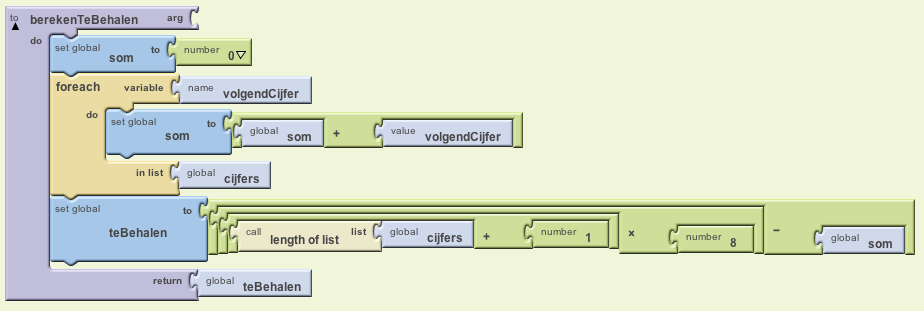
\includegraphics[width=1.4\textwidth]{screenshots/SchrandereScholier_berekenTeBehalen}}
    \caption{\label{screenshots/SchrandereScholier_berekenTeBehalen} Implementatie van berekenTeBehalen}
\end{figure}

De laatste stap is nu een klein stukje toevoegen zodat het te behalen cijfer wordt weergegeven. \marginfig{screenshots/SchrandereScholier_procedureAanroep}{Aanroepen van de bereken procedure}Dit doe je met de blocks in figuur \ref{screenshots/SchrandereScholier_procedureAanroep}. \runOpTelefoon{} Voeg deze blocks toe aan \block{Toevoegen.Click} en test de app uit!

\begin{derivation}{Tip}
Wellicht valt je op dat er ook cijfers in de lijst staan die je niet via de app hebt ingevoerd? Als dit zo is dat heb je in de Blocks Editor nog invulling staan bij het aanmaken van de lijst. Haal deze weg en probeer het opnieuw!
\end{derivation}

\section{Facultatieve uitbreidingen}
Je hebt ondertussen waarschijnlijk al een hoop uitbreidingen op deze app bedacht. Voeg een aantal van de onderstaande functies toe, of bedenk een eigen functie in overleg met jouw docent.

\begin{itemize}
  \item Een 8 gemiddeld, Waarom geen 9? Laat de gebruiker zelf kiezen welk cijfer hij gemiddeld wil staan.
  \item Niet alle toetsen tellen even zwaar, zorg ervoor dat de gebruiker het gewicht van een toets kan bepalen.
  \item Geef de app een mooier uiterlijk.
  \item Zorg ervoor dat de cijfers worden bewaard bij het opnieuw opstarten van de app
  \item Maak de app geschikt voor meerdere vakken.
  \item Maak het onmogelijk om foutieve cijfers in te voeren.
  \item Jouw idee\dots
\end{itemize}